% Sample file on how to use subfiles.
\documentclass[ExampleMasters.tex]{subfiles}

\begin{document}
\clearpage
{\pagestyle{empty}\cleardoublepage}%
\chapter{Discussion (3-4 Seiten)}
\label{chap:discussion}

\section{Results from bench testing}
\label{sec:results_bench}

\begin{itemize}
	\item lessons-learned?
	\item adaptation for future projects
	\item what was taken over for further tests? 
	\item what couldnt be simultaed?
\end{itemize}

\section{Results from processing time evaluation}
\label{sec:results_processing_time}

\begin{itemize}
	\item diagrams (over amplitude, show time)
	\item explain different curves
	\item explain data gathering
	\item mention ramp input 
	\item show reaction time
\end{itemize}
\begin{figure*}[!hbt]
	\centering
	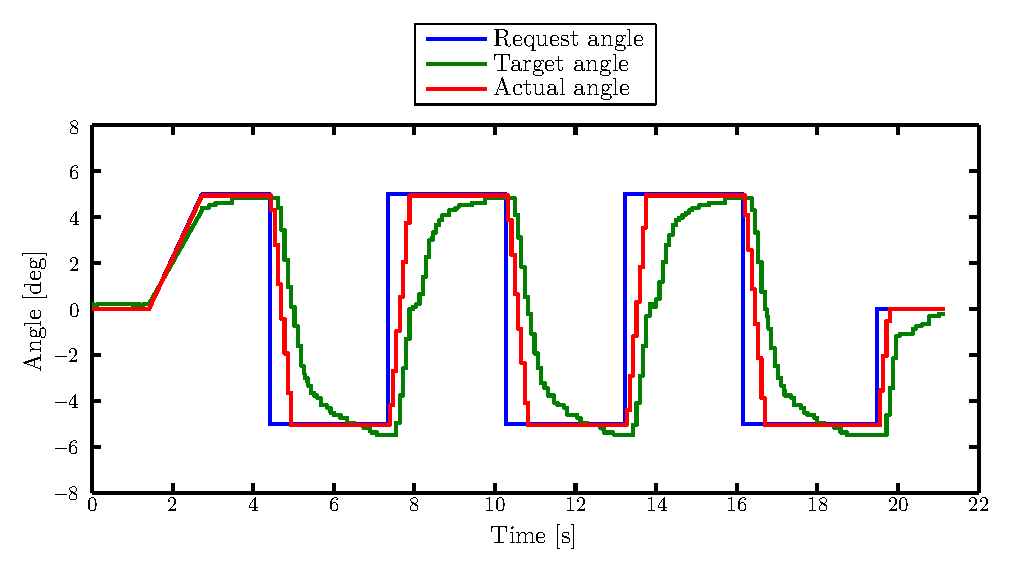
\includegraphics[width=1\linewidth]{figures/lifted_front_5deg}
	\caption{Step input 5 degree}
	
	\label{fig:step_input}
\end{figure*}
During plot analysis of preliminary results it was discussed, whether it would be possible to by-pass the occuring delay by feeding a ramp-input instead of a step-input into the \gls{ETS}. It was assumed that there is a low-pass filter in place which would not affect ramp inputs. Subsequent tests with ramp inputs with varying slopes and amplitudes showed that it was indeed possible to eliminate the low-pass filter leading to no delay between the target angle and the request angle. Nevertheless it was not possible to get any faster change than with the request of a step input. It thus can be concluded that the maximum steering rate of $5 ^\circ /s$ can not be circumvented.
\begin{figure*}[!hbt]
	\centering
	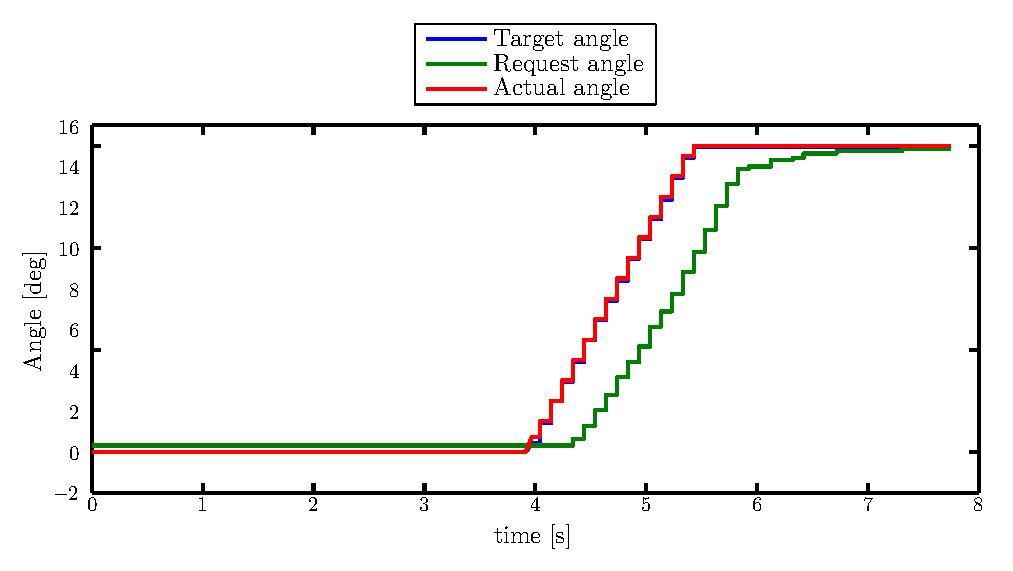
\includegraphics[width=1\linewidth]{figures/rate_limiter1}
	\caption{Step input with rate limiter}
	
	\label{fig:rate_limiter1}
\end{figure*}
\begin{figure*}[!hbt]
	\centering
	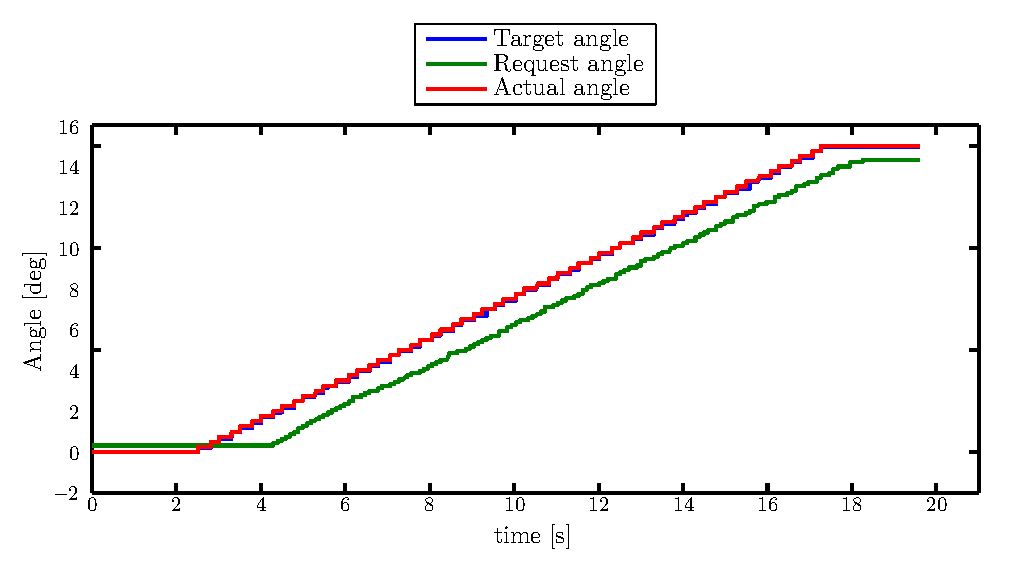
\includegraphics[width=1\linewidth]{figures/rate_limiter2}
	\caption{Low rate input}
	
	\label{fig:rate_limiter2}
\end{figure*}

\begin{figure*}[!hbt]
	\centering
	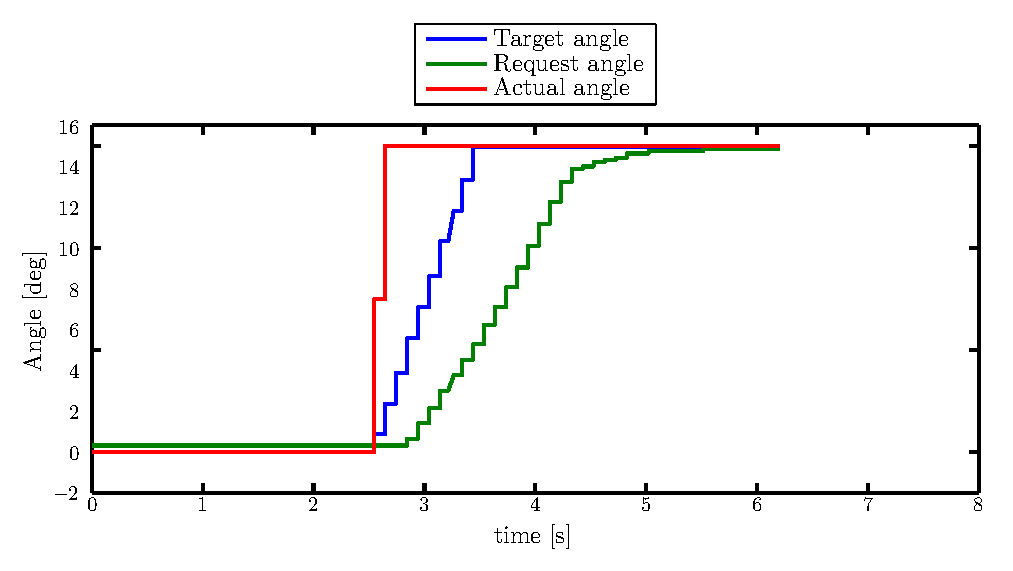
\includegraphics[width=1\linewidth]{figures/rate_limiter4}
	\caption{High rate input}
	
	\label{fig:rate_limiter4}
\end{figure*}


\section{Results from in vehicle testing}
\label{sec:results_vehicle_testing}




\begin{itemize}
	\item CAN-analysis
	\item robustness?
	\item reliability of safety features
\end{itemize}
\section{Results from hardware-in-the-loop testing}

Figure \ref{fig:HIL002_front} shows the measurements of the ETS-CAN of the front axle of the dolly for the low-speed maneuver described in section \ref{sec:HIL}.\\

\begin{figure*}[!htb]
	\centering
	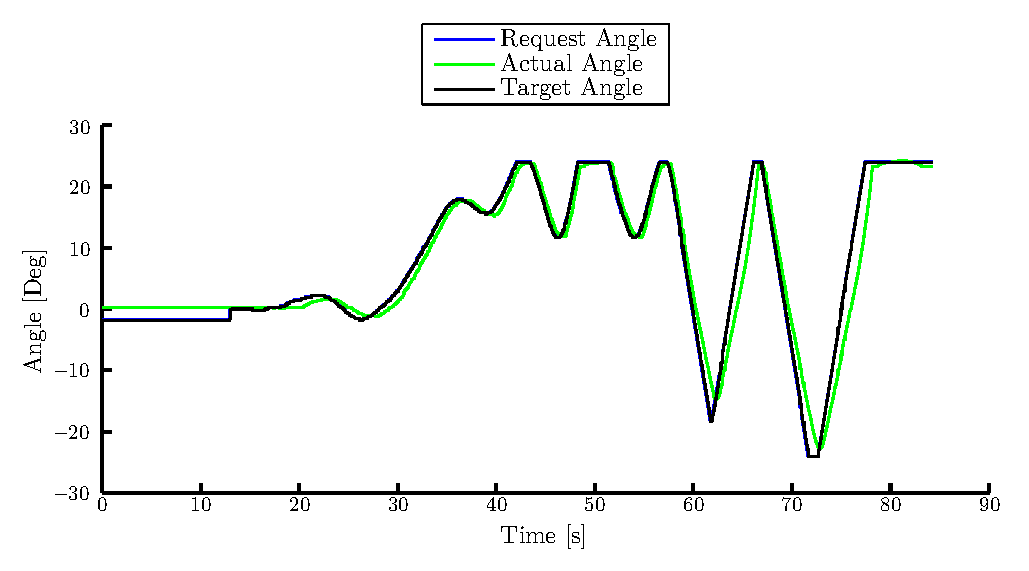
\includegraphics[width=1\linewidth]{figures/HIL002_front}
	\caption{HIL-test low-speed front axle}
	
	\label{fig:HIL002_front}
\end{figure*}

The request angle is the angle that was requested from the controller and then sent from the simulation-PC to the MABII. The target angle is the angle that was calculated by the ETS-ECU and sent as a request to the actuators of the dolly. The actual angle is the angle that the sensors on the dolly's wheels measured.
Figure \ref{fig:HIL002_rear} shows the same measurements for the rear axle.

\begin{figure*}[!htb]
	\centering
	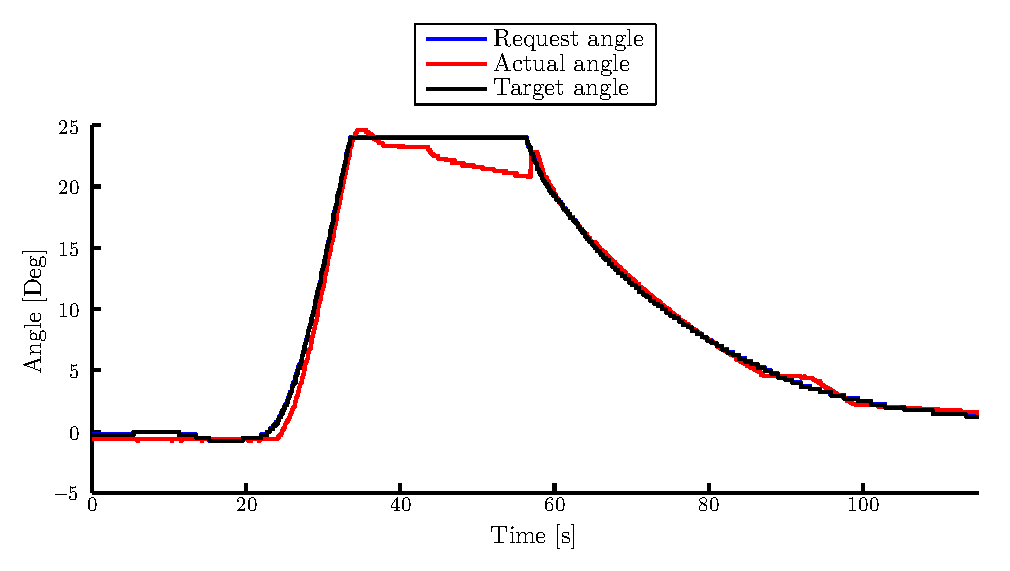
\includegraphics[width=1\linewidth]{figures/HIL002_rear}
	\caption{HIL-test low-speed rear axle}
	
	\label{fig:HIL002_rear}
\end{figure*}
Since the same requested angle for front and rear is the same, below only the front axle is looked upon.
Figure \ref{fig:HIL002_front_closeup} shows an extraction of the measurements of the front axle. 
\begin{figure*}[!htb]
	\centering
	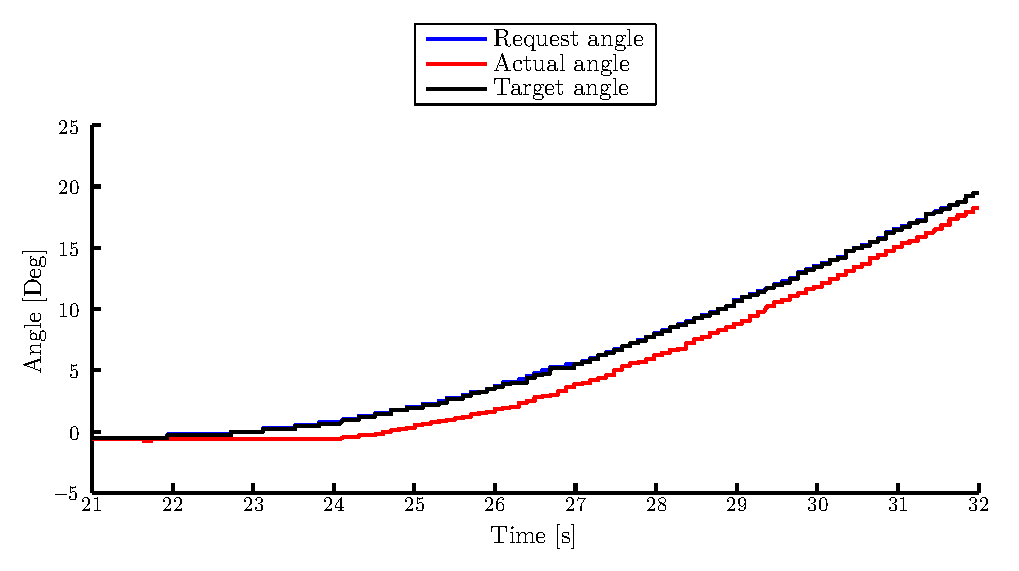
\includegraphics[width=1\linewidth]{figures/HIL002_front_closeup}
	\caption{Details of HIL-test low-speed front axle}
	
	\label{fig:HIL002_front_closeup}
\end{figure*} \\
As already mentioned in section \ref{sec:measuring_delay} there is a delay between the angle requested of the ETS-ECU and the actual angle of the wheels. This can also be seen in this plot. In comparison to this, the delay between the angle request that is sent from the MABII to the CAN and the target angle that is sent from the ETS-ECU to the actuators is very small and can therefore be neglected.\\

To get a picture of the overall results of the HIL-test, Figure \ref{fig:HIL002_complete} shows the measurements conducted on the simulation-PC and the measurements done in ControllDesk in the same plot.  
\begin{figure*}[!htb]
	\centering
	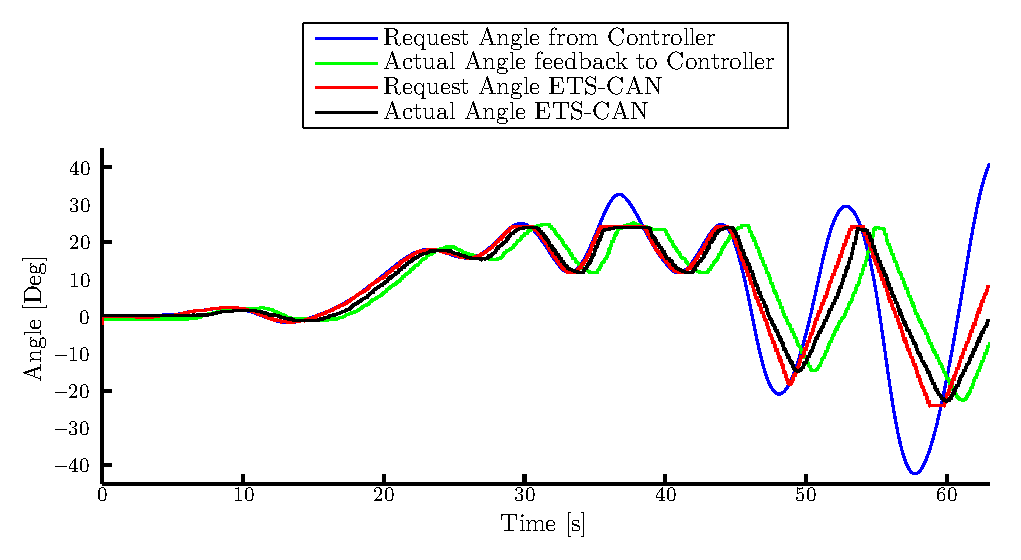
\includegraphics[width=1\linewidth]{figures/HIL002_alles}
	\caption{HIL-test front axle measurements from VTM and ETS-CAN}	
	\label{fig:HIL002_complete}
\end{figure*}

For one thing the plot shows the limitation of the angle that is requested from the controller by the supervisor block described in section \ref{sec:warning_system}. For another thing it shows that there is a relatively high delay between the signal of the actual angle of the dolly from the ETS-CAN and the signal that is feedback to the simulation-PC. This is most likely caused by the use of the serial interface to transmit the signal from the CAN to the simulation-PC. This delay causes a amplification of the articulation angle between the first semitrailer and the dolly, which directly correlates to the steering angle request to the dolly. This amplification can be seen in the end of the measurements.\\
To get a more detailed view of this delay as well as the limitation of the request angle Figure \ref{fig:HIL002_complete_details} shows a extraction of Figure \ref{fig:HIL002_complete}.   

\begin{figure*}[!htb]
	\centering
	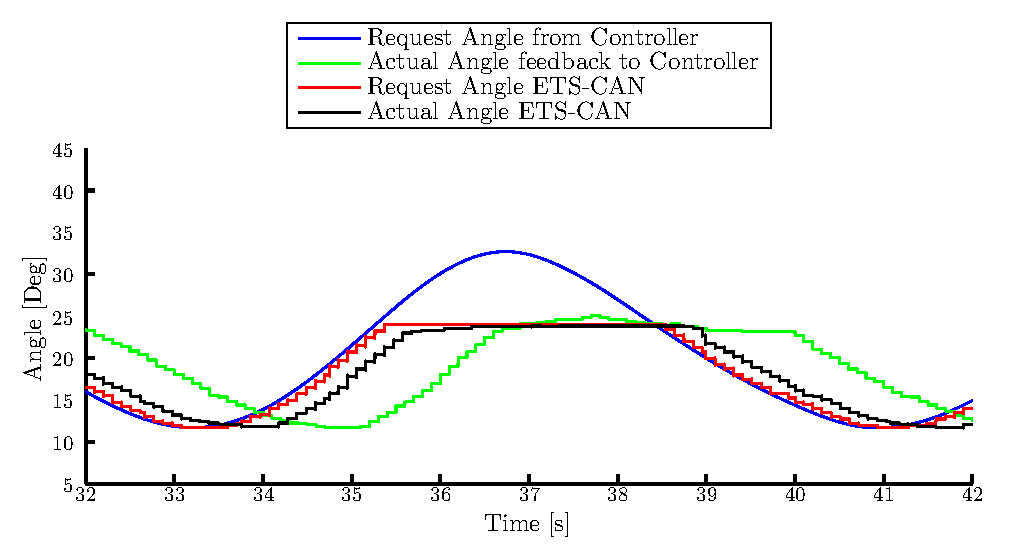
\includegraphics[width=1\linewidth]{figures/HIL002_alles_details}
	\caption{Details of HIL-test front axle measurements from VTM and ETS-CAN}
	
	\label{fig:HIL002_complete_details}
\end{figure*}



\begin{itemize}
	\item compare plots from \gls{HIL}  with simulation
\end{itemize}


\section{Comparison}
\label{sec:results_comparrison}
\begin{itemize}
	\item \gls{VTM}  $<=>$ testing
\end{itemize}







\end{document}
